\documentclass{siproblemset}

\usepackage{multicol}
\usepackage{xcolor}

\newcommand{\der}[2][]{\frac{\text{d}#1}{\text{d}#2}}
\newcommand{\dder}[2][]{\dfrac{\text{d}#1}{\text{d}#2}}
\newcommand{\ddx}[1][]{\frac{\text{d}#1}{\text{d}x}}
\newcommand{\dddx}[1][]{\dfrac{\text{d}#1}{\text{d}x}}

% SI Session Information
\course{MTH 1321}
\sessionnum{8}
\sessiondate{9/30/19}

\warmup{Overview of Basic Derivative Rules}
\topic{Simple Applications of the Derivative}
\topic{Evaluating Derivatives}
\cooldown{Properties of the Derivative}

% Worksheet Information
\title{Basic Derivative Rules}
\sections{Section 3.3}
\withnamespace

\begin{document}
    \maketitle
    
    \activity{Warmup}{Basic Derivative Rules}{Work with a \textbf{partner} to answer these questions. Try not to use your notes.}{15 minutes}
    
    \mcq[2]{Evaluate the following:}{
        \task $\dddx \left[ c\right] $
        \task $\dddx \left[ x^k\right] $
        \tinyspace
        \task $\dddx \left[cf(x)\right]$
        \task $\dddx \left[ f(x)\pm g(x)\right] $
        \tinyspace
        \task $\dddx \left[ e^x\right] $
        \task $\dddx \left[ a^x\right] $
        \tinyspace
        \task $\dddx \left[f(g)\cdot g(x)\right]$
        \task $\dddx \left[ \sqrt{x}\right] $
        \tinyspace
        \task $\dddx \left[x\right]$
        \task $\dddx \left[ \dfrac1x\right] $
        \tinyspace
        \task $\dddx \left[ \dfrac{f(x)}{g(x)}\right] $
        }
    
    \pagebreak
    \activity{Activity 1}{Computing Derivatives Using Derivative Rules}{Make a \textbf{group of two or three, all with the same colored worksheets,} to answer your assigned question. Try not to use your notes.}{30 minutes}
    
    \frq{Find $f'(x)$. Show what derivative rules you use through the process.}
    $$f(x)=x^3e^{x+2}$$
    \largespace
    \mcq{Compute the derivative.}{
        \task $\left[ (2x-9)\left(4e^x+1\right) \right]'$
        \smallspace
        \task $f(x)=\dfrac{2^x}{x^2+1}$
        \smallspace
        \task $f(x)=x^2(3+x^{-1})$
        \smallspace
        \task $\dder[z]{t}\Bigr|_{t=3},~~z=\dfrac{-1}{10-t}$
        \smallspace
        \task $\dder[y]{x}\Bigr|_{x=2},~~y=\left(t-8t^{-1}\right)\left(e^t+t^2\right)$
        \smallspace
        \task $\dddx\left[ \left(\sqrt x - 1\right)\left(\sqrt x + 1\right)\right] $
        \smallspace
        \task $f(x)=\dfrac{x^4+e^x}{x+1}$
        \smallspace
        \task $\left[x^{3/5}e^{5/3}\right]'$
        \smallspace
        \task $g(u)=\dfrac{u+1}{e^u}$
        \smallspace
    }

    \activity{Activity 2}{Applications of Derivatives}{Make a \textbf{{\em new} group of three, all with the different colored worksheets,} to answer these questions. Try not to use your notes.}{30 minutes}
    
        \frq{Find the points on the graph of the curve $y=\dfrac23x^3-5x-4$ at which the tangent line is parallel to $y=3x-2$}
        \mediumspace

    \begin{multipartquestion}
        Determine an equation for the line perpendicular to the tangent line to the curve $y=4x^2-x$ at $(2,14)$.
        \mediumspace
    \end{multipartquestion}

    \begin{multipartquestion}
        Use the following table to find the derivatives.
        
        \begin{center}
            \begin{tabular}{ |c|c|c|c|c|c| }
                \hline
                $f(3)$ & $f'(3)$ & $g(3)$ & $g'(3)$ & $h(3)$ & $h'(3)$ \\
                \hline
                $5$ & $3$ & $-2$ & $6$ & $1$ & $-7$\\
                \hline
            \end{tabular}
        
        \frq{$(fg)'(3)$ and $(f/g)'(3)$}
        \smallspace
        \frq{$\left[ (x+2)f(x)\right]'\Bigr|_{x=3} $}
        \nospace
        \frq{$G'(x)$ where $G(x)=(g(x))^2$}
        \nospace
        \frq{$\dder{x}\left[ f(x)g(x)h(x)\right] $}
        \end{center}
        
    \end{multipartquestion}
\pagebreak
    
    \activity{Cooldown}{Properties of the Derivative}{Attempt to do these problems \textbf{alone} then discuss your answers with the people around you.}{15 minutes}
    \mcq[2]{What is the derivative of the following functions?}{
        \task $f(x)=mx+b$
        \task $g(t)=ct^2$
    }
    \nospace
    \frq{Determine the intervals when the derivative of the following function is positive, negative, and zero.}
    
    \makebox[\width][c]{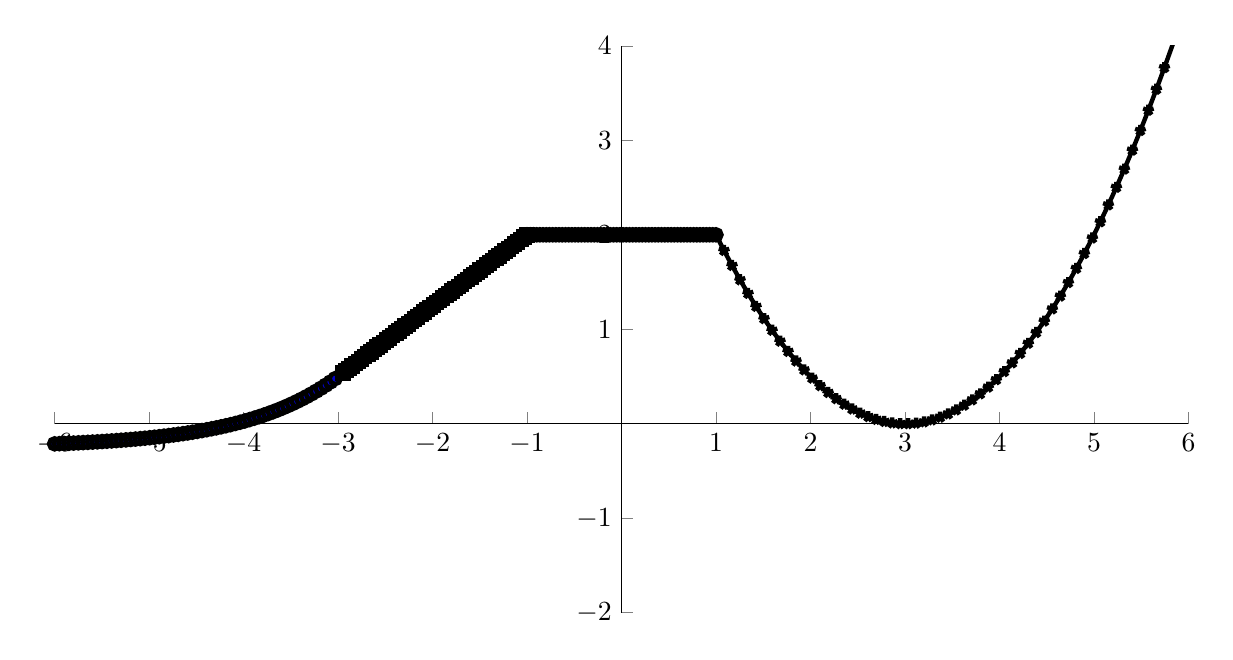
\begin{tikzpicture}[baseline=(current bounding box.north)]
        \begin{axis}[
        x=1.2cm,
        y=1.2cm,
        xmin=-6,
        xmax=6,
        ymin=-2,
        ymax=4,
        axis x line*=middle,
        axis y line*=middle,
        every axis plot/.append style={ultra thick},
        samples=60
        ]
        \addplot+[black, domain=-6:-3.03, restrict y to domain=-10:10] {e^(x+3+ln(3/4))-3/4+0.5};
        \addplot+[black, domain=-2.95:-1] {3/4*x+3/4+2};
        \addplot+[black, domain=-1:1] {2};
        \addplot+[black, domain=1:6] {1/2*(x-3)^2};
        \node at (-3,0.5) {$\circ$};
        \node at (-1,2) {\textbullet};
        \node at (1,2) {\textbullet};
        \end{axis}
        \end{tikzpicture}}
    \mediumspace
    
    \frq{When a function is increasing, it's derivative is \underline{\hspace{2in}}.}
    \frq{When a function is decreasing, it's derivative is \underline{\hspace{2in}}.}
\end{document}